
\chapter{大脑}

\section{了解我们的大脑}

大脑由140亿~230亿个脑细胞组成。
对于常人来说,在这么多的脑细胞中,最多只有15\%左右的脑细胞在参与工作,还有85\%处于待使用状态。
许多为人类发展作出了伟大贡献的科学家和伟人,最多也只使用了20\%的脑细胞。

我们的大脑主要分为左·右大脑半球。
左半脑主要负责逻辑,记忆,实践,语言,判断,排列,分类,分析,书写,推理,抑制,五感等,思维方式具有连续性、衍生性和分析性。
因此左脑可以称为“意识脑”或者”学术脑”。
右半脑主要负责空间形象记忆、直觉、情感、身体协调、视知觉、美术、音乐节奏、想象、灵感、顿悟等,思维方式具有无序性、跳跃性、直觉性等。
因此右脑又称为“创造脑”或者“艺术脑”。


\section{超级记忆里的三个指标}

\begin{itemize}
\item 记忆的速度
\item 记忆的准确度
\item 记忆的持久度
\end{itemize}


\section{记不住的原因}

记不住的原因主要有以下几个方面:
\begin{itemize}
\item 没有找到正确的记忆方法
\item 压力导致容易紧张\\
  从心理学的角度讲,虽然说适度的紧张可以有助于我们提高记忆力,但是过度的紧张会让我们的记忆水平无法很好地发挥。
  克服紧张,只有一个办法,那就是保持乐观积极的心态,多参加有益身心的社团活动,多训练自己当众演讲,增强自己的抗压能力,以减少紧张的次数。
\item 疾病和药物的原因\\
  由于现代医学的发展和各种生物技术的突飞猛进,由药物引发的记忆障碍发生的几率相当的少。
\item 吸烟及过度的饮酒
\end{itemize}



\section{记忆}

1234 -> 140 ~ 230 亿个脑细胞。

左学术,右艺术。
\begin{figure}[H]
  \centering
  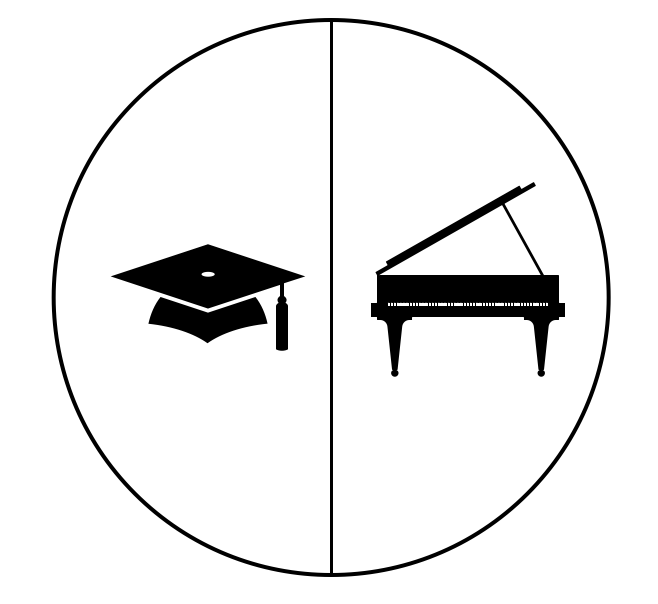
\includegraphics[width=0.6\textwidth]{left-right}
  \caption{左右脑}
\end{figure}

超级记忆三指标:箭矢\argument{速度}飞过,\argument{准确}命中犬夜叉,\argument{持久}定在树上。
\begin{figure}[H]
  \centering
  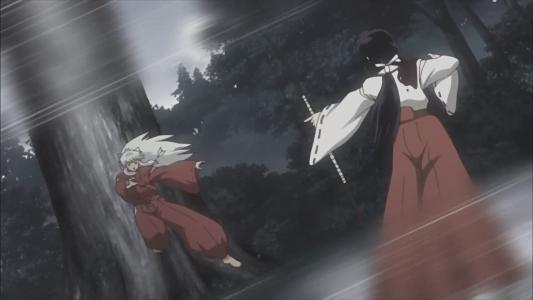
\includegraphics[width=0.8\textwidth]{three-standard}
  \caption{超级记忆三指标}
\end{figure}


记不住的原因:打开\argument{门(方法)},我在\argument{举重(压力)},在\argument{输液(药物)},旁边有禁止\argument{烟酒}的牌子。

\begin{tcolorbox}
脑细胞用\argument{钥匙(14)}打开\argument{中国(23)}的大门。
\argument{左}边有座\argument{物理(学术)}学院,\argument{右}边有座\argument{艺术}学院。
艺术学院在考记忆绘画:箭矢\argument{速度}飞过,\argument{准确}命中犬夜叉,\argument{持久}定在树上。
物理学院的学生刚考完\argument{几部著(记不住)}作,打开\argument{门(方法)},看到我在\argument{举重(压力)},并且在\argument{输液(药物)},旁边还有禁止\argument{烟酒}的牌子。


\end{tcolorbox}

%%% Local Variables:
%%% mode: latex
%%% TeX-master: "memory"
%%% End:
